%%
% La siguiente plantilla esta basada en el siguiente enlace:
% http://academic.reed.edu/physics/courses/Physics332.s08/reports.html
% La plantilla original puede descargarse de ese sitio
% Se dejo parte del texto original en inglés para ilustar el uso de la plantilla
% Se hicieron algunas modificaciones para ajustar el idioma y otros detalles para 
% completar un reporte técnico breve pero muy puntual
% Modificación Inicial: Marco Aurelio Nuno Maganda - 11/SEP/2014
% 
% Enlace a la documentación del tipo de documento base (revtex4)
% http://mirror.hmc.edu/ctan/macros/latex/contrib/revtex/doc/latex/revtex/source/revtex4-1.pdf
%
% En algunas distribuciones es necesario instalar el paquete texlive-publishers
%
\documentclass[conference]{IEEEtran}

\usepackage[spanish]{babel}
\usepackage{amsmath,amssymb,amsfonts,amsthm}
\usepackage{graphicx}
\usepackage[utf8]{inputenc}
\usepackage{url}
\usepackage{hyperref}
\usepackage{balance}

\graphicspath{{figuras/}{./}}

%%%%%%%%%%%%%%%%%%%%%%%%%%%%%%%%%%%%%%%%%%%%%
% PARCHE PARA ELIMINAR LA FECHA DEL DOCUMENTO
\usepackage{etoolbox}
\makeatletter
\patchcmd{\frontmatter@RRAP@format}{(}{}{}{}
\patchcmd{\frontmatter@RRAP@format}{)}{}{}{}
\makeatother
% FIN DEL PARCHE
%%%%%%%%%%%%%%%%%%%%%%%%%%%%%%%%%%%%%%%%%%%%%

\usepackage[backend=bibtex,sorting=none]{biblatex}
\setcounter{biburllcpenalty}{7000}
\setcounter{biburlucpenalty}{8000}
\addbibresource{references.bib}

\usepackage{datetime}
\newdateformat{specialdate}{\twodigit{\THEDAY}-\twodigit{\THEMONTH}-\THEYEAR}
\date{\specialdate\today}

\usepackage[hyphenbreaks]{breakurl}

\renewcommand\spanishtablename{Tabla}
\renewcommand\spanishfigurename{Figura}

\hypersetup{
    hidelinks,
    colorlinks=false,
    pdfborder={0 0 0}
}

\begin{document}

\newcommand{\breite}{1.0}

% ============================================
% TITULO Y AUTORES (ORDEN ALFABETICO)
% ============================================
\title{Migración del demo de la Pinacoteca a Jetpack Compose con renderizado OpenGL ES}

\author{\IEEEauthorblockN{Bañuelos Rodríguez Guillermo Saúl\IEEEauthorrefmark{1},\quad
Castillo Treto Juan Carlos\IEEEauthorrefmark{1},\\
Gutiérrez Gómez Veyra María\IEEEauthorrefmark{1},\quad
Hernández Medina César Alejandro\IEEEauthorrefmark{1},\quad
Vargas Cepeda Emiliano\IEEEauthorrefmark{1}}
\IEEEauthorblockA{\IEEEauthorrefmark{1}Ingeniería en Tecnologías de la Información\\
Universidad Politécnica de Victoria\\
Equipo 6 - Proyecto 6}
}

\maketitle

\begin{abstract}
El desarrollo de aplicaciones de realidad virtual y recorridos virtuales en Android tradicionalmente se ha realizado utilizando el framework de vistas XML y OpenGL ES para el renderizado 3D \cite{wright2010}. Con la llegada de Jetpack Compose como el toolkit moderno de interfaz de usuario declarativa \cite{android_compose}, surge la necesidad de migrar aplicaciones existentes a este nuevo paradigma sin perder la funcionalidad gráfica avanzada. En este trabajo se presenta la migración del demo de la Pinacoteca de la Universidad Politécnica de Victoria ---una aplicación de recorrido virtual con renderizado OpenGL ES, control mediante sensores de rotación y soporte para gamepad--- desde el modelo tradicional de actividades con XML hacia Jetpack Compose \cite{compose_viewinterop}. Se describe el proceso de integración de GLSurfaceView dentro del árbol composable mediante AndroidView, la corrección de la navegabilidad con controles físicos \cite{android_gamepad}, la limitación del ángulo de cabeceo para evitar movimientos fuera de plano \cite{android_sensors}, y la preservación de la reproducción de audio y el manejo del ciclo de vida. La aplicación migrada mantiene la funcionalidad original del demo y mejora la fluidez del desplazamiento con el control.
\end{abstract}

\section{Introducción}

Los recorridos virtuales y las aplicaciones de visualización arquitectónica en 3D han encontrado en los dispositivos móviles una plataforma accesible y portátil para su ejecución \cite{wright2010,shreiner2013}. La Universidad Politécnica de Victoria cuenta con un demo de realidad virtual de la Pinacoteca desarrollado en Java sobre Android, que permite al usuario desplazarse por el modelo tridimensional del edificio utilizando los sensores de rotación del dispositivo para orientar la cámara y un gamepad o los controles táctiles para el movimiento \cite{android_sensors}.

Con la introducción de Jetpack Compose como el toolkit recomendado para nuevas interfaces de usuario en Android, se vuelve relevante migrar las aplicaciones existentes a este paradigma declarativo, el cual simplifica la creación de UI, reduce el código boilerplate y facilita el mantenimiento \cite{android_compose}. Sin embargo, Compose no reemplaza directamente a OpenGL ES, por lo que la integración de gráficos 3D requiere el uso de mecanismos de interoperabilidad como AndroidView para embeber un GLSurfaceView tradicional dentro de la jerarquía composable \cite{compose_viewinterop}.

El presente proyecto, asignado al Equipo 6 como parte de la Unidad I de Programación Móvil, tiene como objetivo migrar el demo de la Pinacoteca a Jetpack Compose, corrigiendo además dos problemas presentes en la versión original: la navegabilidad con el control y el movimiento fuera de plano al voltear hacia arriba \cite{android_gamepad}. En las siguientes secciones se describe la arquitectura de la aplicación migrada, el modelo de renderizado con OpenGL ES, la composición de la escena 3D, el manejo de sensores y controles, y las correcciones implementadas.

\section{Desarrollo Experimental}

\subsection{Arquitectura de la aplicación migrada}

La aplicación migrada conserva la misma lógica de renderizado OpenGL ES de la versión original, encapsulada en la clase CubeRenderer, pero reemplaza el sistema tradicional de Activities con layouts XML por una única Activity que utiliza Jetpack Compose para definir la interfaz. La integración del GLSurfaceView se realiza mediante el componente AndroidView, que permite embeber una View del framework clásico dentro del árbol de composición \cite{compose_viewinterop}.

La Figura~\ref{fig:arquitectura} muestra la estructura de componentes principales de la aplicación migrada. La actividad principal (MainActivity) extiende ComponentActivity e implementa SensorEventListener para recibir las lecturas del sensor de rotación. La interfaz se define en la función composable PinacotecaScreen, que contiene un AndroidView encargado de crear y gestionar el GLSurfaceView. El renderizado 3D está a cargo de CubeRenderer, que implementa GLSurfaceView.Renderer. De forma complementaria, la actividad maneja los eventos de gamepad mediante onGenericMotionEvent y onKeyDown, y gestiona la reproducción de audio con MediaPlayer.

\begin{figure}[!ht]
\centering
\includegraphics*[width=0.7\columnwidth]{diagrama1}
\caption{Arquitectura de la aplicación migrada. La actividad principal implementa SensorEventListener y maneja los eventos de gamepad. La UI se define con Compose y embebe el GLSurfaceView mediante AndroidView.}
\label{fig:arquitectura}
\end{figure}

\subsection{Renderizado OpenGL ES}

El renderizado de la escena 3D de la Pinacoteca se realiza con OpenGL ES 2.0 a través de la clase CubeRenderer, que implementa GLSurfaceView.Renderer \cite{android_opengl}. Esta clase gestiona la carga y compilación de shaders GLSL (vertex y fragment shader) para el mapeo de texturas mediante ShaderHelper, la carga de texturas desde recursos drawable mediante TextureHelper, y la construcción de la escena mediante operaciones de matriz de modelo (pushMatrix, popMatrix, traslaciones). El renderizado es estereoscópico con dos viewports (izquierdo y derecho) para compatibilidad con visores de realidad virtual \cite{opengl_docs}.

La escena se compone de cuatro zonas principales, como se ilustra en la Figura~\ref{fig:escena}: un cielo envolvente formado por cinco planos con textura de cielo, una base de césped como plano de piso, la estructura arquitectónica exterior de la Pinacoteca con sus paredes, entrada principal y techo, y el salón interior que contiene obras de arte en sus paredes, un piso de madera y una puerta de acceso.

\begin{figure}[!ht]
\centering
\includegraphics*[width=0.9\columnwidth]{diagrama4}
\caption{Composición de la escena 3D de la Pinacoteca. Se muestran las cuatro zonas principales y las texturas utilizadas en cada una.}
\label{fig:escena}
\end{figure}

El salón interior es la zona con mayor detalle, compuesto por 14 segmentos de piso con textura de madera, 4 segmentos de techo, 7 segmentos en la pared izquierda con texturas de obras de arte (izq\_1 a izq\_6), 7 segmentos en la pared derecha con pinturas (der\_1 a der\_6), 2 segmentos en la pared frontal y 2 en la pared de espalda. En total, la escena utiliza 34 texturas diferentes cargadas desde los recursos de la aplicación.

\subsection{Integración con Jetpack Compose}

La integración entre OpenGL ES y Jetpack Compose se logra mediante el componente AndroidView dentro de la función composable PinacotecaScreen. Este componente recibe una factory que crea el GLSurfaceView, configura la versión de EGL (2.0), asigna el renderer y establece el modo de renderizado continuo (RENDERMODE\_CONTINUOUSLY) \cite{compose_viewinterop}.

El manejo del ciclo de vida del GLSurfaceView se realiza con DisposableEffect, que llama a onResume() al entrar en composición y a onPause() al salir, coordinándose con los callbacks onResume() y onPause() de la Activity para el registro y baja del sensor de rotación. Esta sincronización es crítica para evitar fugas de memoria y asegurar que el sensor no continúe activo cuando la aplicación está en segundo plano \cite{deitel2017}.

\subsection{Manejo de sensores y orientación}

La orientación de la cámara se controla mediante el sensor TYPE\_ROTATION\_VECTOR, que proporciona la matriz de rotación del dispositivo. En el callback onSensorChanged() se obtiene la matriz de rotación, se re-mapea el sistema de coordenadas intercambiando los ejes X y Z para adaptar la orientación del dispositivo al sistema de coordenadas de OpenGL, y se extraen los ángulos de orientación (azimuth, pitch, roll) que se pasan al renderer mediante el método setOrientation() \cite{android_sensors}.

\subsection{Corrección de navegabilidad y control de movimiento}

Se realizaron dos correcciones principales sobre la versión original:

\textbf{1) Navegabilidad con control físico:} Se incrementó la velocidad de desplazamiento con el D-Pad de 10 a 15 unidades por evento, y con el joystick analógico de 3 a 5 unidades. La velocidad de giro con el joystick derecho se incrementó de 10 a 15 grados por evento, logrando una respuesta más ágil y natural al navegar por la escena \cite{android_gamepad}.

\textbf{2) Limitación del movimiento fuera de plano:} En el callback onSensorChanged() se agregó una restricción al ángulo de cabeceo (pitch), limitándolo a un máximo de 1.2 radianes (aproximadamente 70 grados). La Figura~\ref{fig:pitch} muestra el diagrama de flujo de esta corrección. Esto evita que la cámara voltee completamente hacia arriba o hacia abajo, lo que en la versión original provocaba que el usuario perdiera la orientación espacial y saliera del plano de navegación.

\begin{figure}[!ht]
\centering
\includegraphics*[width=0.7\columnwidth]{diagrama2}
\caption{Diagrama de flujo de la corrección del ángulo de cabeceo (pitch). Se limita el ángulo vertical a un máximo de 1.2 radianes para evitar que la cámara salga del plano de navegación.}
\label{fig:pitch}
\end{figure}

\subsection{Navegación y flujo de datos}

La Figura~\ref{fig:navegacion} ilustra el flujo de datos entre los componentes principales de la aplicación. El sensor de rotación alimenta a MainActivity, que actualiza la orientación en CubeRenderer. Los eventos de gamepad se procesan en onGenericMotionEvent y onKeyDown, invocando los métodos de movimiento del renderer (MoveForward, StrafeRight, RotateX, RotateY). La UI de Compose contiene el GLSurfaceView y se comunica con el renderer a través de la referencia mantenida en la actividad.

\begin{figure}[!ht]
\centering
\includegraphics*[width=0.7\columnwidth]{diagrama3}
\caption{Diagrama de navegación y flujo de datos entre los componentes del sistema. Las flechas continuas indican llamadas directas; las punteadas indican actualizaciones por eventos.}
\label{fig:navegacion}
\end{figure}

\subsection{Audio y ciclo de vida}

La reproducción del audio de fondo se mantiene mediante MediaPlayer con un archivo de audio en bucle. Se gestiona en los callbacks onResume() (iniciar/reanudar), onPause() (pausar) y onStop() (liberar recursos), coordinado con el ciclo de vida del GLSurfaceView para evitar fugas de memoria \cite{deitel2017}.

\section{Resultados}

La aplicación migrada se ejecutó en un dispositivo Android físico para verificar 
el correcto funcionamiento de todas sus funcionalidades. La interfaz se renderiza 
correctamente en Compose, mostrando el GLSurfaceView a pantalla completa con el 
renderizado estereoscópico funcional.

\begin{figure}[!ht]
\centering
\includegraphics*[width=0.6\columnwidth]{pinacoteca-exterior}
\caption{Vista exterior de la Pinacoteca durante la navegación con la aplicación migrada.}
\label{fig:exterior}
\end{figure}

\begin{figure}[!ht]
\centering
\includegraphics*[width=0.6\columnwidth]{pinacoteca-interior}
\caption{Vista del interior del salón de la Pinacoteca mostrando las obras de arte 
en las paredes.}
\label{fig:interior}
\end{figure}

La orientación de la cámara responde al sensor de rotación del dispositivo. Al girar físicamente el teléfono, el usuario puede mirar en cualquier dirección horizontal (360 grados) mientras que la mirada vertical queda limitada a aproximadamente 70 grados hacia arriba y hacia abajo. Esta limitación corrige efectivamente el problema de movimiento fuera de plano que presentaba la versión original.

El desplazamiento con el D-Pad del gamepad se volvió más ágil: los movimientos de avance, retroceso y desplazamiento lateral responden con mayor rapidez, permitiendo recorrer la escena de forma más natural. El joystick analógico también presenta una respuesta mejorada, tanto en el modo de movimiento como en el modo de giro. El audio de fondo se reproduce en bucle y se pausa correctamente al minimizar la aplicación, reanudándose al regresar a ella.

No se detectaron fugas de memoria ni caídas de rendimiento durante sesiones de uso prolongadas, lo que confirma que la integración entre Compose y OpenGL ES mediante AndroidView es estable para aplicaciones de recorrido virtual.

\subsection{Problema detectado y corrección implementada}

Durante las pruebas de funcionamiento de la aplicación se identificó que el renderizado estereoscópico presentaba únicamente dos vistas rectangulares correspondientes al ojo izquierdo y derecho, sin incorporar un marco que simulara la visualización a través de un visor de realidad virtual. Aunque la escena tridimensional se mostraba correctamente y el recorrido era funcional, la ausencia de este elemento visual disminuía la sensación de inmersión y hacía que la interfaz se percibiera como una simple división de pantalla en lugar de una experiencia orientada a dispositivos de realidad virtual.

Para resolver este problema se implementó un marco gráfico alrededor de cada una de las vistas estereoscópicas. La incorporación del marco mejoró la presentación visual de la aplicación y permitió que la visualización se asemejara al comportamiento esperado de un visor tipo Google Cardboard, proporcionando una experiencia más inmersiva sin afectar el funcionamiento del motor de renderizado OpenGL ES ni el desempeño general de la aplicación.

La Figura~\ref{fig:marco_vr} muestra la evidencia de la corrección implementada, donde se observa el marco incorporado alrededor de las dos vistas estereoscópicas del recorrido virtual.

\begin{figure}[!ht]
\centering
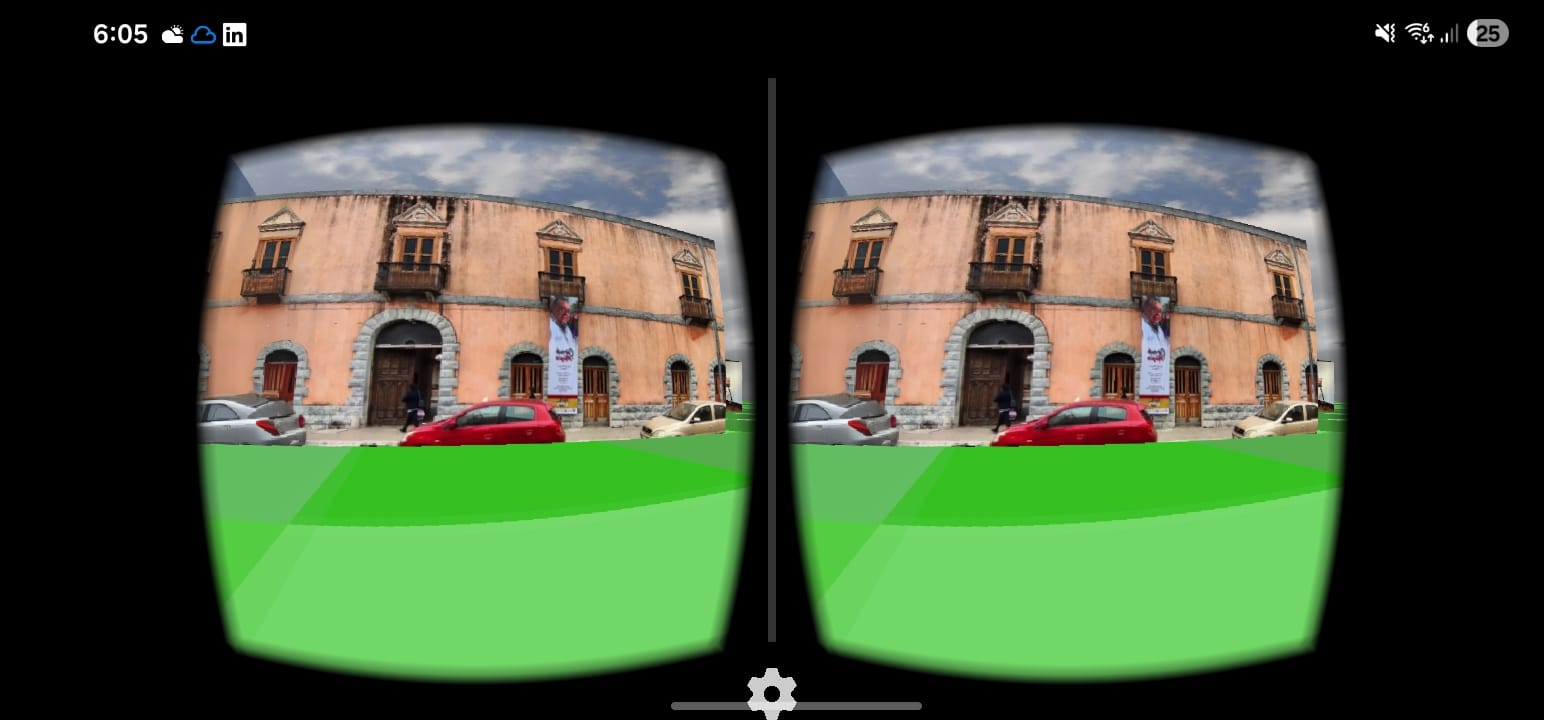
\includegraphics[width=0.85\columnwidth]{marco_vr}
\caption{Evidencia de la implementación del marco para el visor de realidad virtual.}
\label{fig:marco_vr}
\end{figure}

\section{Conclusión}

En este trabajo se realizó la migración exitosa del demo de la Pinacoteca de la UPV desde el modelo tradicional de Android con XML hacia Jetpack Compose, manteniendo la funcionalidad completa de renderizado 3D con OpenGL ES, control por sensores y soporte para gamepad. La integración de GLSurfaceView mediante AndroidView demostró ser un mecanismo efectivo para conservar el código de renderizado existente sin necesidad de reescribirlo \cite{compose_viewinterop}.

Se corrigieron dos problemas importantes de la versión original: la navegabilidad con el control físico, que ahora responde con mayor velocidad y fluidez, y el movimiento fuera de plano al voltear hacia arriba, resuelto mediante la limitación del ángulo de cabeceo a 1.2 radianes \cite{android_sensors}. Estas correcciones mejoran significativamente la experiencia de usuario durante la navegación por el recorrido virtual.

Como trabajo futuro se plantea migrar completamente el renderizado a un enfoque nativo de Compose utilizando GraphicsLayer, lo que eliminaría la dependencia de AndroidView, y agregar soporte para nuevos edificios del campus universitario como el Edificio C y las cafeterías \cite{horton2021,phillips2022}.

\addcontentsline{toc}{section}{Referencias}
\printbibliography

\end{document}